\lstset{language=Java,
numberstyle=\footnotesize,
basicstyle=\ttfamily\footnotesize,
frame=shadowbox,
breaklines=true}

\section*{Task 2 - Lucene}

\subsection*{Oppgave a}

Kode lagt til i \textit{MyDocument.java}.
\lstinputlisting[language=Java, firstline=10, lastline=41]{src/ir/MyDocument.java}

\noindent Kode endret i \textit{MyIndexFiles.java}.
\lstinputlisting[language=Java, firstline=21, lastline=41]{src/ir/MyIndexFiles.java}

\noindent Output fra kommandovinduet ved kjøring av \textit{MyIndexFiles.main()} etter modifisering av kode.
\begin{lstlisting}[frame=single]
Usage: java org.apache.lucene.demo.IndexFiles <root_directory>
Indexing to directory 'index'...
adding /Users/hakloev/git/TDT4117/oving4/20news-part/40008
adding /Users/hakloev/git/TDT4117/oving4/20news-part/40027
adding /Users/hakloev/git/TDT4117/oving4/20news-part/40062
... 
for alle 1907 dokumentene
...
adding /Users/hakloev/git/TDT4117/oving4/20news-part/59648
adding /Users/hakloev/git/TDT4117/oving4/20news-part/59652
Optimizing...
1811 total milliseconds

Process finished with exit code 0
\end{lstlisting}

\newpage
\subsection*{Oppgave b}

\begin{figure}[p]
\centering
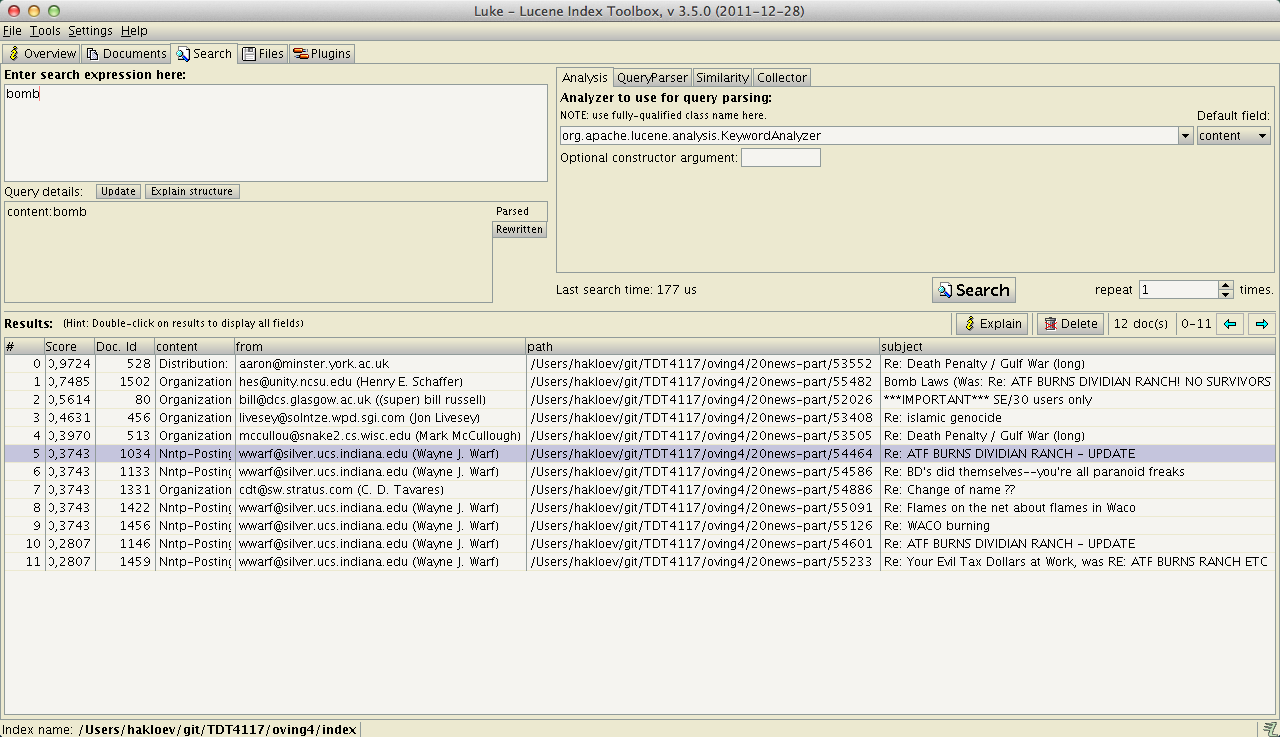
\includegraphics[scale=0.31]{images/bombcontent.png}
\caption{Søk etter bomb i content}
\end{figure}

\begin{figure}[p]
\centering
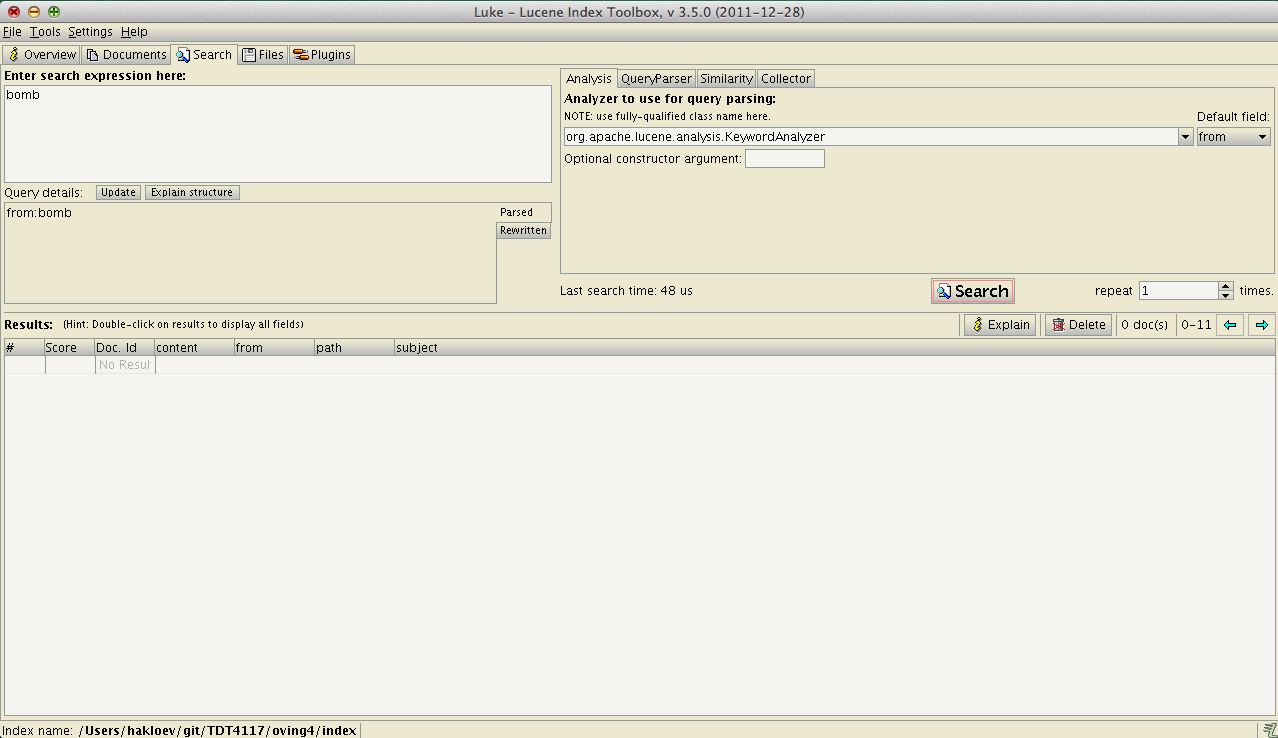
\includegraphics[scale=0.31]{images/bombfrom.png}
\caption{Søk etter bomb i from}
\end{figure}

\begin{figure}[p]
\centering
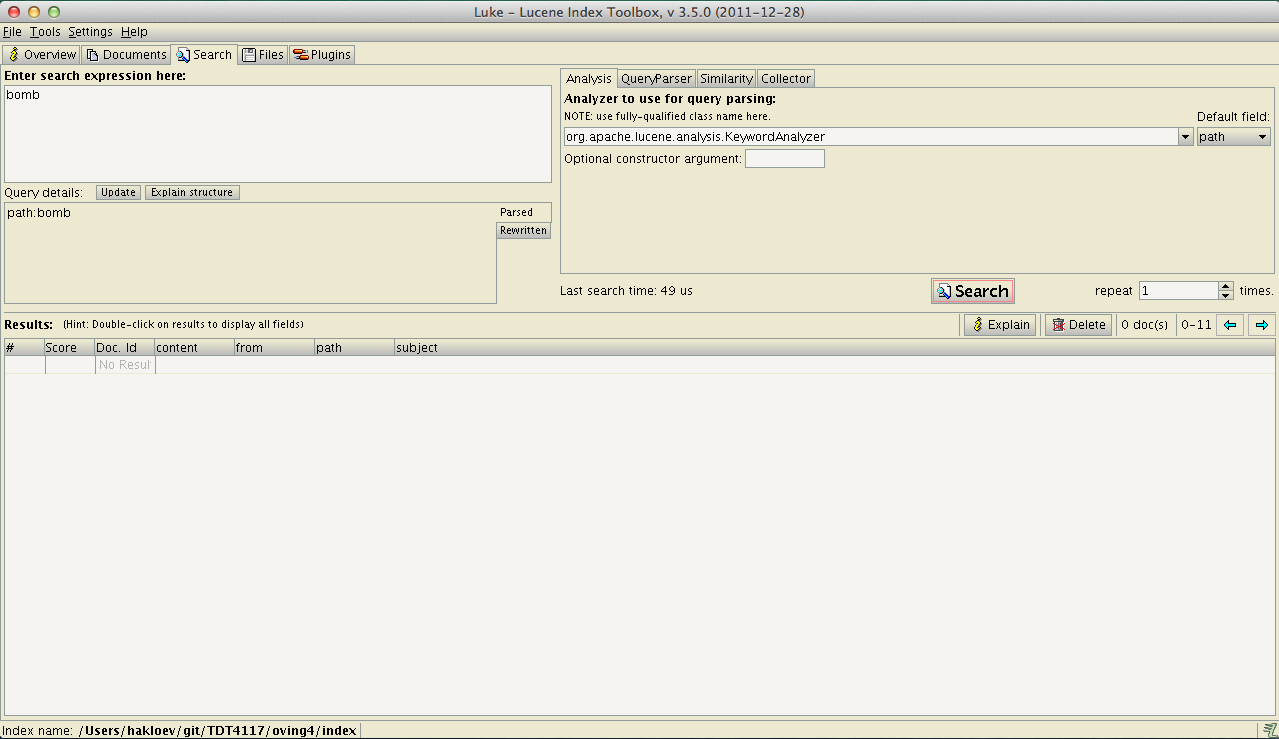
\includegraphics[scale=0.31]{images/bombpath.png}
\caption{Søk etter bomb i path}
\end{figure}

\begin{figure}[p]
\centering
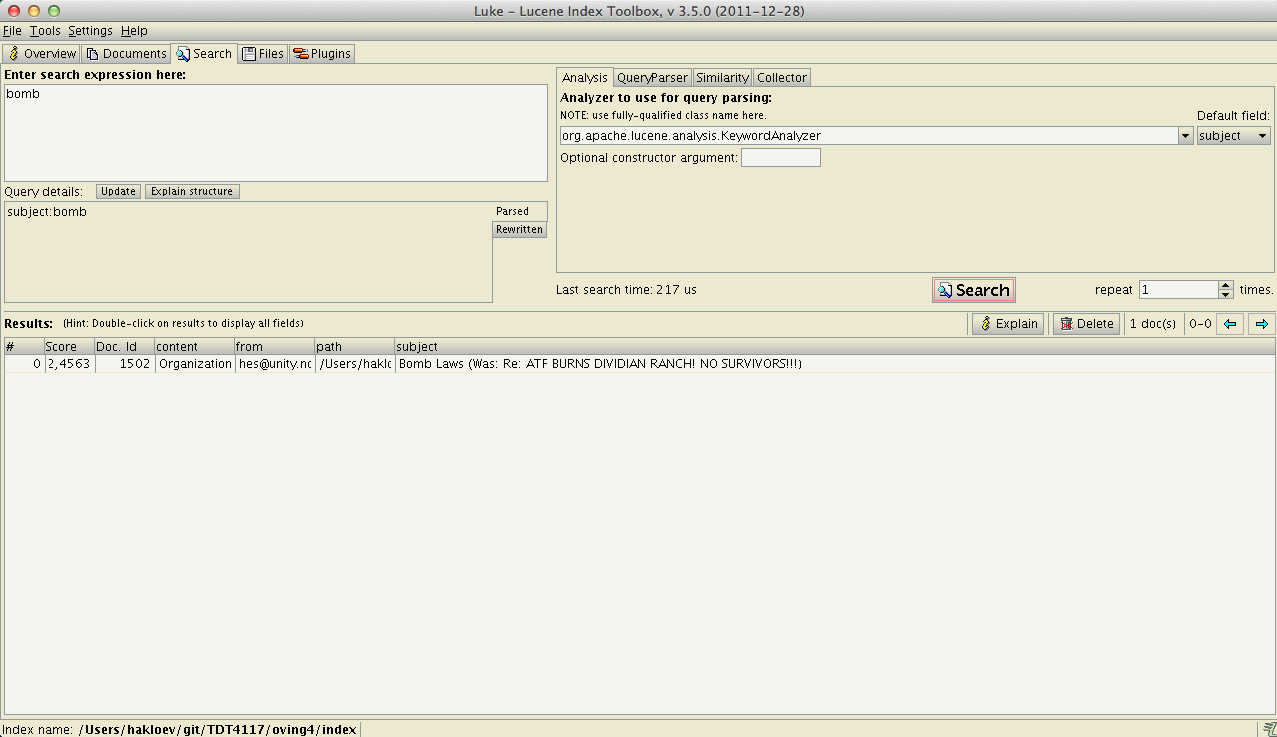
\includegraphics[scale=0.31]{images/bombsubject.png}
\caption{Søk etter bomb i subject}
\end{figure}

\subsubsection*{Forklaring av systemet}
